\setchapterpreamble[u]{\margintoc}
\chapter{Estimating radiometric data from synthetic LiDAR}
\labch{lidar_intensity}
\label{sec:lidar_intensity}

\section*{About this chapter}

This chapter estimates intensity data over the previously explained \acrshort{lidar} simulator. Semantic labels have been previously mentioned as additional data that provide further insight into the observed materials. However, there are other properties which are estimated during flight and also help to characterize materials, such as the return intensity. Hence, surfaces can be modelled with \acrshort{brdf}s to estimate intensity, multiple returns, return losses, etc. At least two approaches exist for modelling \acrshort{brdf}s. The trivial one is to consider the traditional Computer Graphics \acrshort{brdf}s, whereas a more up-to-date solution consists of utilizing \acrshort{brdf} databases measured from real-world surfaces with a gonio-photometer. Another alternative is to transfer \acrshort{lidar} data into \acrshort{dl} models to estimate the intensity from the observed depth. However, the latter approach requires solving the \acrshort{lidar} simulation in the image space. Other approaches are based on the voxelization of point clouds, thus losing part of the details of the scene, or using, for instance, graph-based representations for point clouds. Nevertheless, \acrshort{dl}-based alternatives are out of the scope of this dissertation and thus only the first two explained approaches will be evaluated in this section.

Comparisons with previous work are not trivial to establish, nor against real-world scans, since the latter requires having the model of a real-world scene that should be scanned with real and synthetic \acrshort{lidar}. As a consequence, the discussion of this chapter is merely focused on the modelling of scenarios with distinct materials. This way, the intensity histograms can be evaluated to check whether both approaches achieve similar results as well as the differences between \acrshort{tls} and \acrshort{als}. For instance, the intensity distribution is expected to be correlated to the viewing angle and thus on the kind of scan, either terrestrial or airborne. Similarly, some materials are expected to return higher intensity values, in comparison with other materials with a dull appearance.

This chapter explains the two mentioned approaches for estimating \acrshort{lidar} intensity, based on the work of Chapter \ref{sec:lidar_simulation}. Both approaches, together with the required parameters, are depicted in Figure \ref{fig:lidar_intensity_overview}.

\section{On the estimation of LiDAR intensity}

The most straightforward approach for simulating \acrshort{lidar} intensity is to use traditional shading functions, also called analytical \acrshort{brdf}s. The number of possible \acrshort{brdf}s is very limited, or at least, these are not enough to emulate any real-world material. Furthermore, these are typically constrained to estimating red, green and blue data with rendering-based material properties, including the albedo colour and specular factors. Other \acrshort{brdf}s have a larger number of configurable parameters such as the material roughness and reflectivity. However, it is not trivial to determine which \acrshort{brdf} is the most similar to emulate one specific material in a synthetic scenario. For instance, both Oren-Nayar and Lambertian \acrshort{brdf}s have a dull appearance.

\begin{figure}
    \centering
    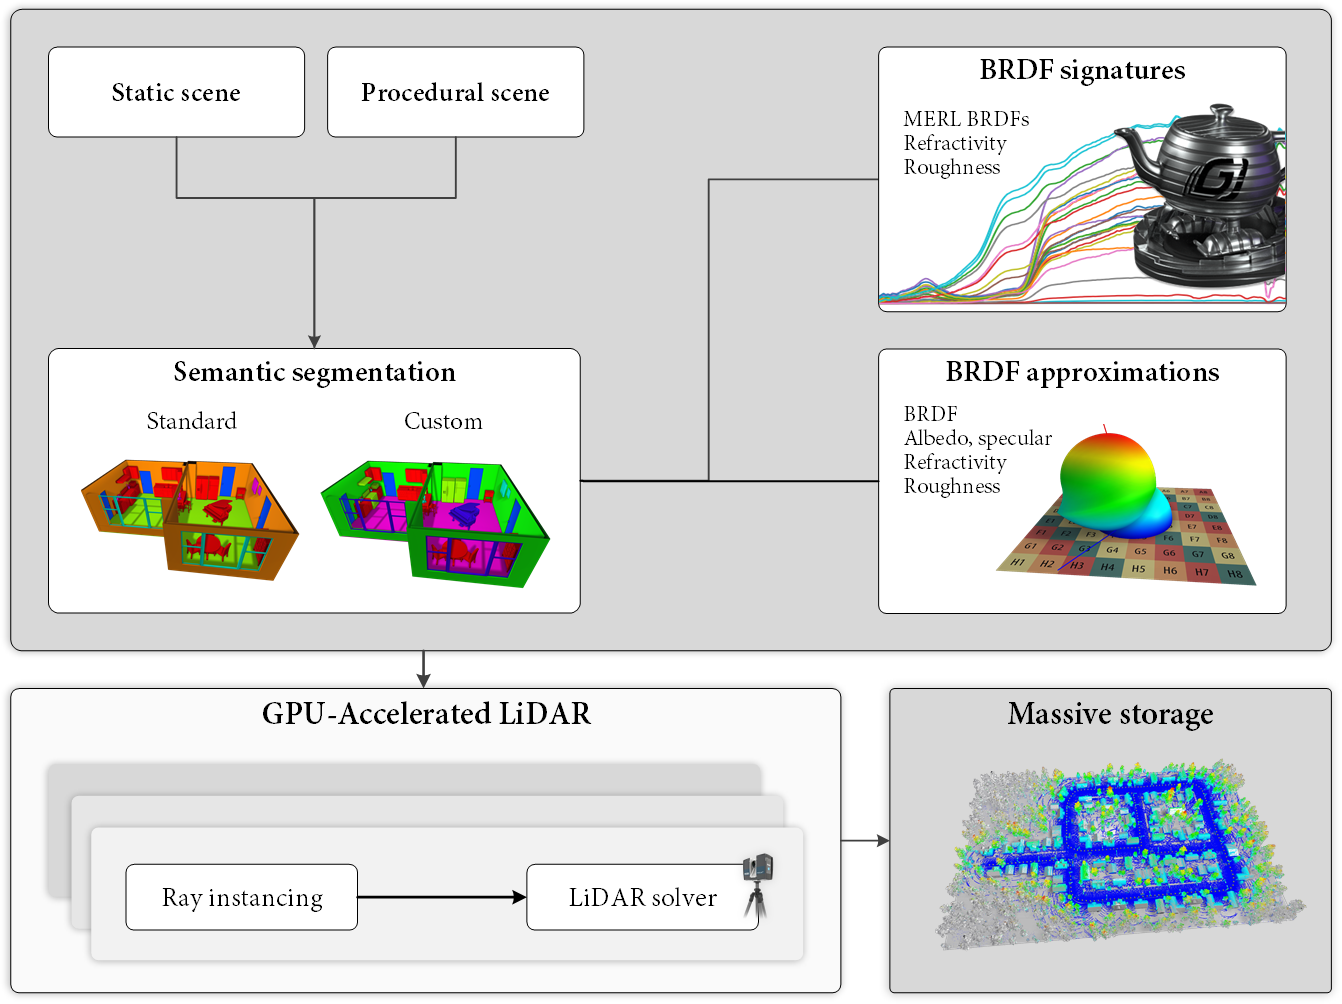
\includegraphics[width=\linewidth]{figs/lidar_intensity/overview.png}
    \caption{Overview of the proposed \acrshort{lidar} simulation. First, the input scenarios are attached to semantic annotations and materials. Then, the previously explained \acrshort{lidar} simulator solves the scan and the resulting point cloud is stored in a standard file format.}
	\label{fig:lidar_intensity_overview}
\end{figure}

More recently, Dupuy and Jakob \cite{dupuy_adaptive_2018} published a database of spectral signatures from isotropic and anisotropic materials, comprising the interval ranging from 358.628 \si{\nano\meter} to 1001.89 \si{\nano\meter} with a sampling frequency of $\sim$3.341 \si{\nano\meter}. On the other hand, previous databases were limited to red, blue, and green wavelengths as they were designed for rendering applications \cite{matusik_data-driven_2003}. From these very first databases, other studies were able to parameterize the collected materials to build a larger database \cite{serrano_intuitive_2016}. However, \acrshort{rgb} databases are not appropriate for simulating most of nowadays sensors as they may operate in a wavelength interval that is not included in the \acrshort{rgb} spectra. For instance, infrared devices cannot be simulated with \acrshort{rgb} data. Still, state-of-the-art hyperspectral databases cannot help to simulate every kind of \acrshort{lidar}. A frequent wavelength in \acrshort{lidar} technology is 1550 \si{\nano\meter}, which is not covered by the signatures collected by Dupuy and Jakob \cite{dupuy_adaptive_2018}. Hence, \acrshort{brdf} databases are improving by covering wider spectra, including the infrared, though are still not sufficient for other kinds of sensors such as \acrshort{lidar}. Still, this approach is more physically accurate than the first one, despite being limited to wavelengths below 1000 \si{\nano\meter}.

A brief insight into the literature on the simulation of radiometric data shows the confusion between ray-tracing and ray-casting concepts. To the best of our knowledge, none of the previous \acrshort{lidar} simulators work as a ray-tracing solver. Instead, rays are cast and the collision intensity is estimated \cite{ahn_real-time_2020, zhao_method_2021, bechtold_helios_2016}. However, this fusion of \acrshort{tof} and radiometry estimations has led previous work to erroneously refer to this as ray-tracing. Besides this, the operating wavelength has been barely taken into account in the simulation \cite{chen_analysis_2022, gschwandtner_blensor_2011, zohdi_rapid_2020}. Other works use widespread \acrshort{brdf}s such as Oren-Nayar, Lambert and Blinn-Phong \cite{chen_analysis_2022}. More physically-based approaches use material properties such as diffuse, specular and transmissive factors provided by third-party vendors \cite{haider_development_2022}. Finally, other state-of-the-art methods use images co-acquired with \acrshort{lidar} information to estimate intensity \cite{vacek_learning_2022, xiao_synlidar_2021}. These are typically affected by environmental conditions such as lighting and neither is guaranteed that the material database is large enough. However, the former drawback can be tackled using libraries that help to estimate several environmental and lighting scenarios from a single image \cite{buslaev_albumentations_2020}. Similarly, sensor defects and limitations could be simulated by training a \acrshort{dl} model \cite{guillard_learning_2022}.  
\section{Material modelling}

\begin{figure*}
    \centering
    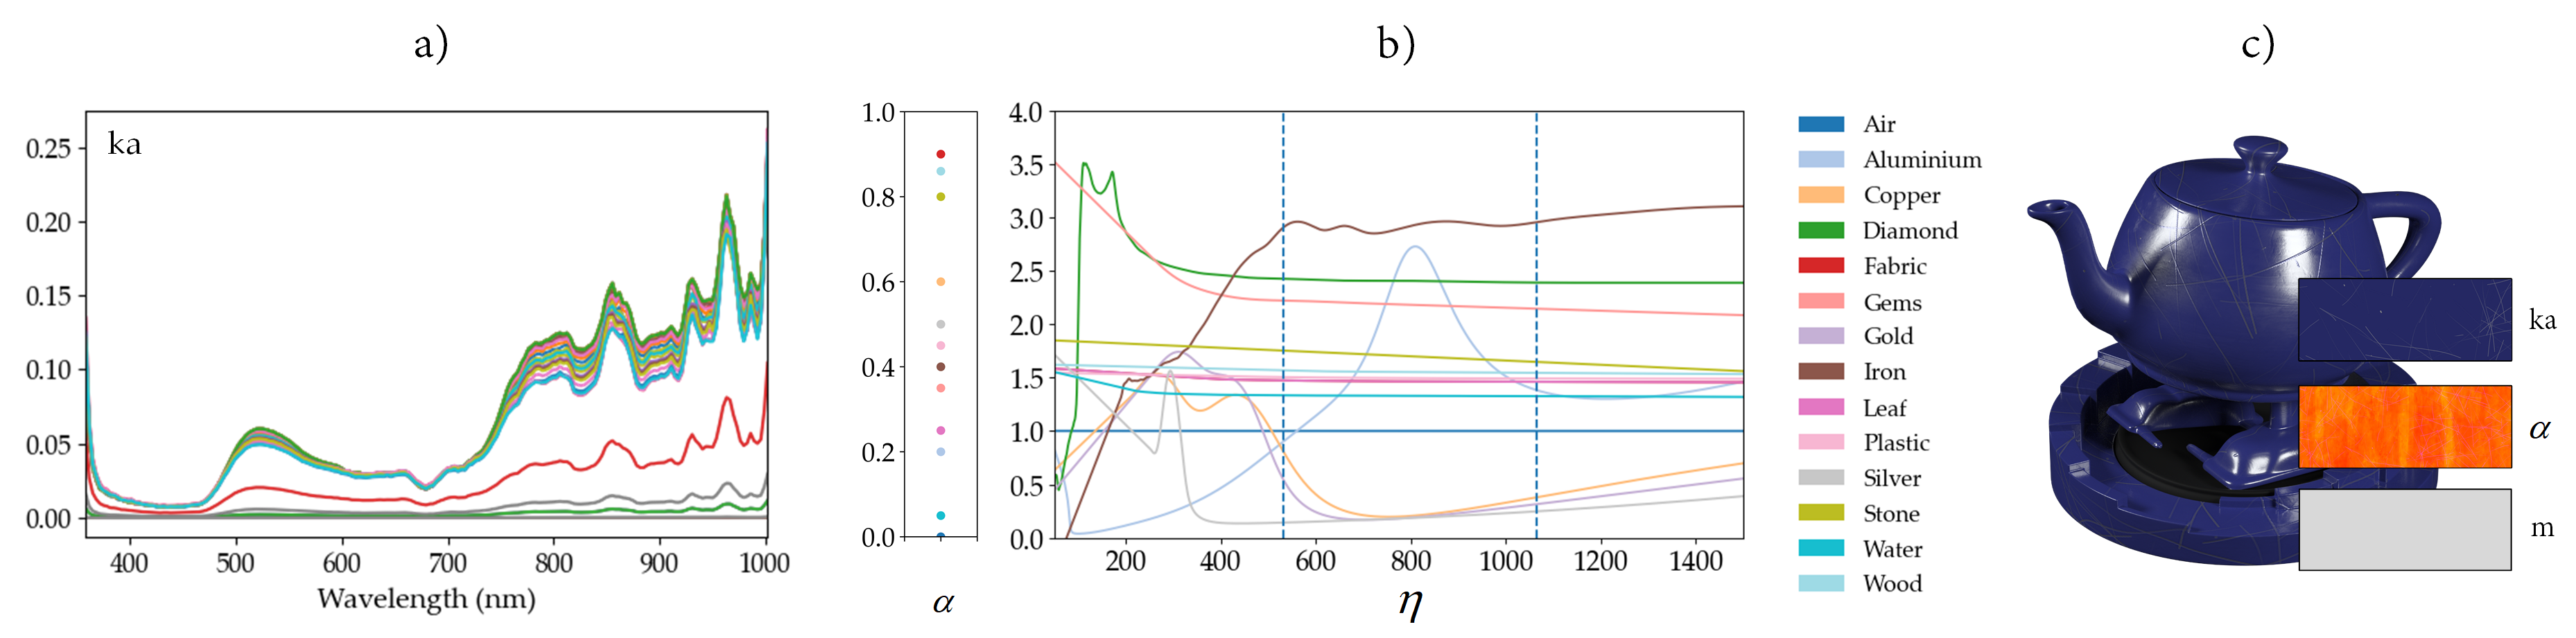
\includegraphics[width=\linewidth]{figs/lidar_intensity/brdf_properties.png}
	\caption{Modelling of scene surfaces to estimate the returned intensity. a) Reflectance from a \acrshort{brdf} parameterized with the input and output vector ($w_i$ and $w_o$) \cite{dupuy_adaptive_2018} and b) model-agnostic material specifications, including refractivity and roughness exponent. Finally, c) previous material properties are scaled according to the model textures (albedo, metallic and roughness). }
	\label{fig:lidar_brdf_properties}
\end{figure*}

Static and procedural models are linked to semantic annotations and materials that help to calculate the \acrshort{lidar} intensity. As previously proposed, materials and any other kind of data can be attached to models following a hierarchical search based on the object's name and its material name. The latter is used if the object's name is not unique, i.e., it collides with the name of other objects. Rather than defining the material of every surface from scratch, a material database is provided to facilitate the modelling of surfaces, covering some widespread materials such as stone, fabric, plastic, iron, etc. Each one of these materials is parameterized with at least three properties, as can be observed in Figure \ref{fig:lidar_brdf_properties}. Using the \acrshort{brdf}s collected by a gonio-photometer fastens the calculations as it already provides the reflectance, whereas the shading \acrshort{brdf}s use the albedo and specular colours, among other factors, as part of the formulae. Still, the values obtained from the \acrshort{brdf} database are scaled according to the object's albedo. Also, the refractivity ($\eta$) is required to account for changes in the traversed medium, whereas the roughness ($\alpha \in [0, 1]$) is utilized for modelling return losses. The refractivity is not provided as a value, but rather as the Id of a material in a database of refractive indices. 

The refractive indices were obtained from publicly available signatures collected from a large number of peer-reviewed works \cite{mikhail_n_polyanskiy_refractive_nodate}. In comparison with the sampled \acrshort{brdf}s, refractive indices are provided as sparse values in a variable wavelength range (it varies from one work to another). Therefore, the refractivity signatures are first used to construct a Catmull-Rom spline which can be later sampled for the \acrshort{lidar} wavelength. This property is especially relevant for bathymetric \acrshort{lidar} since the refracted vector is computed according to the refractivity of two different mediums.

\acrshort{brdf}s help to estimate the ratio between incoming and outcoming radiance for a specific wavelength by considering the incidence angle of \acrshort{lidar} beams, regardless of using analytical \acrshort{brdf}s or collected \acrshort{brdf}s. In this stage, the emitter and the receiver are assumed to have the same location, and therefore, incident ($\vec{w_{i}}$) and reflected ($\vec{w_{o}}$) vectors are the same. The latter assumption helps to considerably reduce the memory footprint of the second approach in the \acrshort{gpu}. Omitting this would lead to having $n \times n$ samples instead of $n$, with $n$ being the sampling resolution of the collected signatures in a semisphere. 

\section{Analytical BRDFs}

Analytical \acrshort{brdf}s require some properties that are typically provided as \acrshort{pbr} textures. However, transferring these textures during the simulation either implies solving this piece-wise or building a texture atlas, with the latter having a very limited dimensionality in \acrshort{opengl}. Instead, the albedo, normal, roughness and metallic texture were sampled per vertex before solving the simulations and subsequently stored together with the vertex data. The object-wise texture sampling was efficiently solved using \acrshort{opengl}'s compute shaders.

\begin{figure}
    \centering
    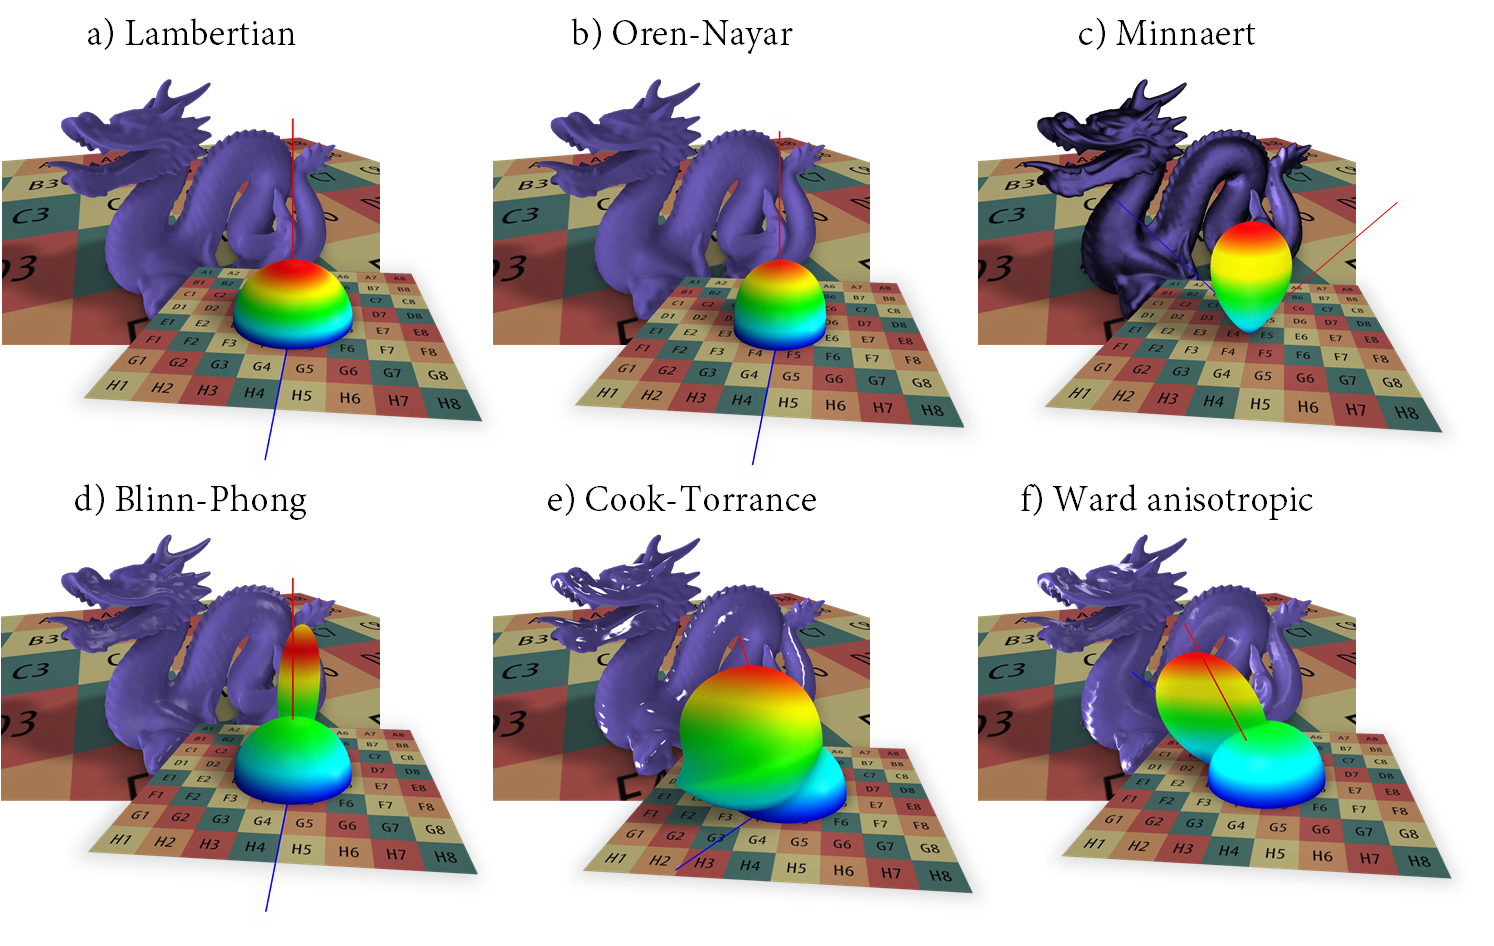
\includegraphics[width=\linewidth]{figs/lidar_intensity/analytical_brdfs.png}
    \caption{\acrshort{brdf}s depicted 1) by shading a 3D model and 2) by distorting a semi-sphere with the estimated intensity. $f_{r}(\vec{w})$ is represented by the distance from each vertex of the distorted semi-sphere to the origin, [0, 0, 0]. From left to right: a) Lambertian, b) Oren-Nayar with $\alpha_{m}$ = 0.5, c) Minnaert with a darkening factor ($k$) of 1.47, whereas $\rho_{d}$ is increased by a factor of A = 2.6, d) Blinn-Phong with $\alpha$ = 11, e) Cook-Torrance with $\alpha$ = 0.685 and $F_{0}$ = 0.40, and f) Ward anisotropic with $\alpha_{x}$ = 0.15 and $\alpha_{y}$ = 0.75. $\rho_{d}$ = 1 for all the illustrations.  }
	\label{fig:lidar_analytical_brdfs}
\end{figure}

The returned reflectance was part of the \acrshort{lidar} equations presented in Chapter \ref{sec:fundamentals_rs}, whereas the overall formula helps to account for other atmospheric and viewing conditions. The focus of this chapter is simply on the returned reflectance, although the intensity reported in later experiments corresponds to the formulae explained in Chapter \ref{sec:fundamentals_rs}. The first approach is to estimate the reflectance with analytical functions, $f_{r}(\vec{w})$, that calculate the amount of light received back to the scanner, according to the incoming energy. In this manner, a \acrshort{brdf} can be used for each type of surface, or so to speak, for each material. In order to cover most of the materials represented in our scenarios, six different \acrshort{brdf}s, depicted in Figure \ref{fig:lidar_analytical_brdfs}, were included. The rendering of the Dragon model shows the aftermath of sampling \acrshort{brdf}s with many view (outgoing) and normal vectors and a single incoming vector from the light. As in the \acrshort{lidar} formulae, the calculated intensity is conditioned by, at least, the dot product between the incoming vector and the surface normal. On the other hand, the semisphere is discretized with a variable resolution, and its vertices were scaled according to the reflectance sampled for a single incoming and outgoing vector, conditioned by the vertex's normal vector. Accordingly, the Lambertian \acrshort{brdf} spreads the same amount of energy in every direction regardless of the surface normal. For the latter representations, reflectance is typically normalized with $1/\pi$ to account for energy spreading.

However, these \acrshort{brdf}s can be simplified whether incident and reflected vectors are assumed to be equal, $w_{i} = w_{o}$. That is, the outgoing \acrshort{lidar} beam and the incoming energy, which reaches the sensor's receiver, have the same direction (. The following formulae show the backscattering form of the \acrshort{brdf} models depicted in Figure \ref{fig:lidar_analytical_brdfs} and described in \cite{montes_soldado_overview_2012, guarnera_brdf_2016}, where $\rho_{d}$ and $\rho_{s}$ are diffuse and specular colors of the material, and $h$ is the halfway vector ($\hat{l} + \hat{v} = 2w_{o}$, where $\hat{l}$ and $\hat{v}$ are light and view vectors, respectively).
\begin{itemize}
    \item Lambertian: 
    \begin{gather}
        \label{eq:lambert_brdf}
        \begin{aligned}
            f_{r}(\vec{w}) = \frac{\rho_{d}}{\pi}
        \end{aligned}
    \end{gather}
    \item Oren-Nayar: 
    \begin{gather}
        \label{eq:oren_nayar_brdf}
        \begin{aligned}
            f_{r}(\vec{w}) &= \frac{\rho_{d}}{\pi}(A + B)\sin{\theta_{w}} \tan{\theta_{w}}\\
            A &= 1 - 0.5 \frac{{\alpha_{m}^{2}}}{{\alpha_{m}}^2 + 0.33}\\
            B &= 0.45 \frac{{\alpha_{m}^{2}}}{{\alpha_{m}}^2 + 0.09}
        \end{aligned}
    \end{gather}
    \item Minnaert:
    \begin{gather}
        \label{eq:minnaert_brdf}
        \begin{aligned}
            f_{r}(\vec{w}) &= \frac{\rho_{d}}{\pi}(\hat{n} \cdot \hat{w})^{2(k-1)}
        \end{aligned}
    \end{gather}
    \item Blinn-Phong: 
    \begin{gather}
        \label{eq:blinn_phong_brdf}
        \begin{aligned}
            f_{r}(\vec{w}) &= \rho_{s}(\hat{n} \cdot \hat{h})^{k} = \rho_{s}(\hat{n} \cdot 2\hat{w})^{k}
        \end{aligned}
    \end{gather}
    \item Cook-Torrance: 
    \begin{gather}
        \label{eq:cook_torrance_brdf}
        \begin{aligned}
            f_{r}(\vec{w}) &= \frac{F(\beta)D(h)G(\vec{w})}{\pi (\hat{n} \cdot \hat{w})^{2}}\\
            F(\beta) &= F_{0} + (1 - F_{0}) (1 - \hat{n} \cdot \hat{w})^{5}\\
            D(h) &= \frac{1}{\alpha^{2}_{m} (\hat{h} \cdot \hat{n})^{4}} \exp{\frac{(\hat{h} \cdot \hat{n})^{2} - 1}{\alpha^{2}_{m}(\hat{h} \cdot \hat{n})^{4}}}\\
            G(w) &= \min\left(1, \frac{4(\hat{n} \cdot \hat{w})^{2}}{\hat{h} \cdot \hat{w} }\right)
        \end{aligned}
    \end{gather}
    where $F(\beta)$ is the Schlick approximation \cite{akenine-moller_real-time_2018}, $D(h)$ is the Beckmann distribution \cite{montes_soldado_overview_2012} and $G(h)$ is the geometric attenuation factor. $F_{0}$ is the external reflection under normal incidence casuistic ($\vec{w} = \vec{n}$), whereas the rest of the values are approximated through interpolation between $F_{0}$ and 1.
    \item Ward anisotropic: 
    \begin{gather}
        \label{eq:ward_brdf}
        \begin{aligned}
            f_{r}(\vec{w}) &= \frac{\rho_{s}\exp\left(-\frac{\left(\frac{h \cdot x}{\alpha_{x}}\right)^{2} + \left(\frac{h \cdot y}{\alpha_{y}}\right)^{2}}{(\hat{h} \cdot \hat{n})^{2}} \right)}{4\pi\alpha_{x}\alpha_{y} (\hat{n} \cdot \hat{w})}
        \end{aligned}
    \end{gather}
\end{itemize}

An example of intensity estimation with analytical \acrshort{brdf}s is shown in Figure \ref{fig:lidar_analytical_brdfs_intensity_result}, with the vehicle path highlighted with yellow lines. 

\begin{figure}[ht]
    \centering
    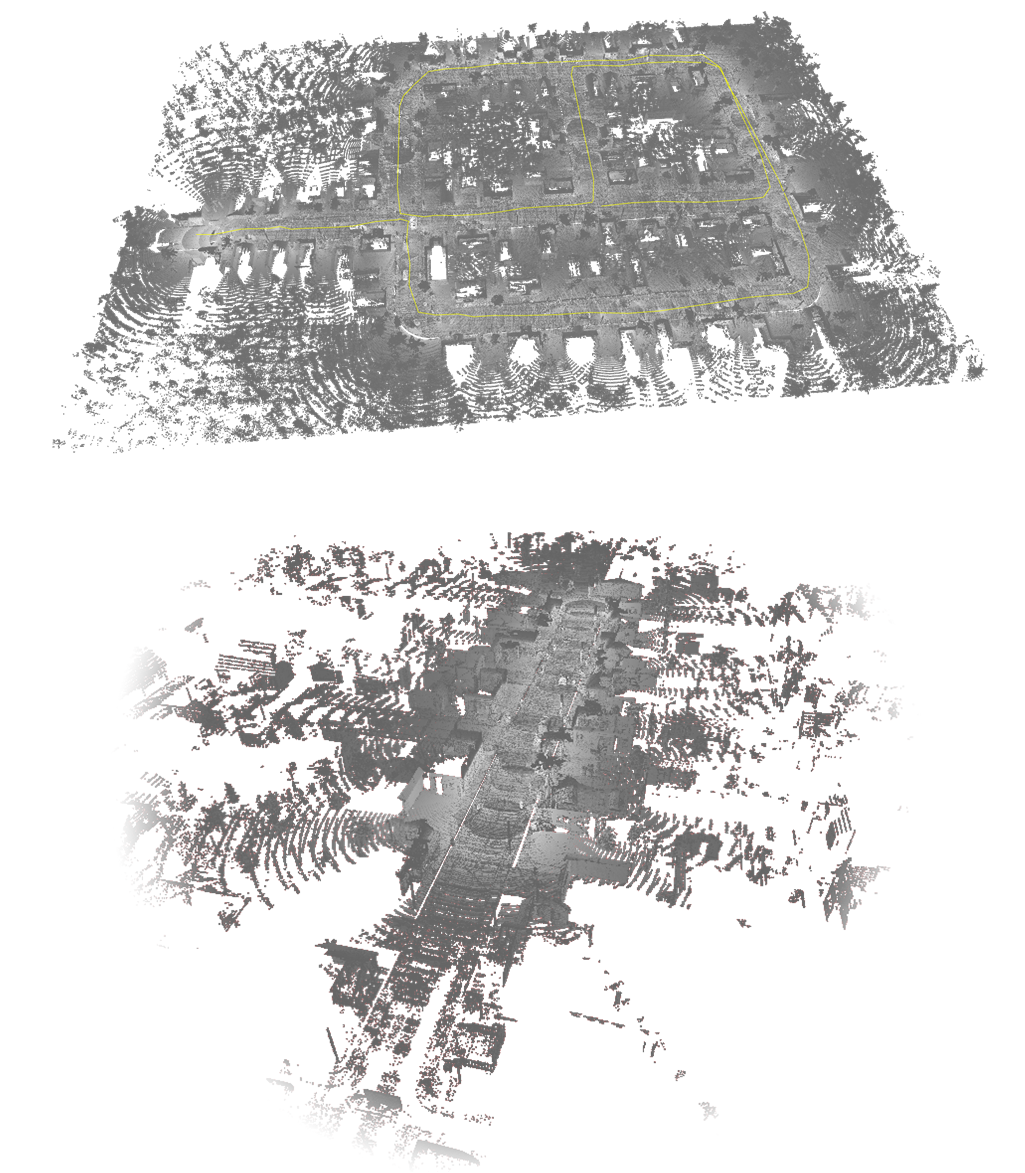
\includegraphics[width=\linewidth]{figs/lidar_intensity/analytical_brdf_intensity_result.png}
    \caption{Intensity simulated using the analytical \acrshort{brdf}s in the scanning of an urban environment. }
	\label{fig:lidar_analytical_brdfs_intensity_result}
\end{figure}

\section{BRDF database}

The main concern when using databases collecting \acrshort{brdf} signatures is to store the discretized representation and to sample it from the \acrshort{lidar} simulation. From the database provided by Dupuy and Jakob \cite{dupuy_adaptive_2018}, a single semisphere sampling was discretized with $360 \times 90 \times 195$ values from spatial and spectral dimensions. These values were queried from the interface published together with the collected materials, which evaluates the database with the incoming and outgoing vectors, $w_i$ and $w_o$, albeit both being equal in our solution. Also, the \acrshort{lidar} wavelength must be linked to the index of the most similar wavelength in the database. Before the simulation, every material is subsampled to store $x \times y$ samples instead of $x \times y \times w$, with $x$ and $y$ are the length of azimuth and elevation discretizations, respectively, and $w$ referring to the spectral dimensionality. Examples of sampled signatures are depicted in Figure \ref{fig:brdf_merl_examples}, using random $w_i$ and $w_o$ vectors.

\begin{marginfigure}[-2.0cm]
    \centering
    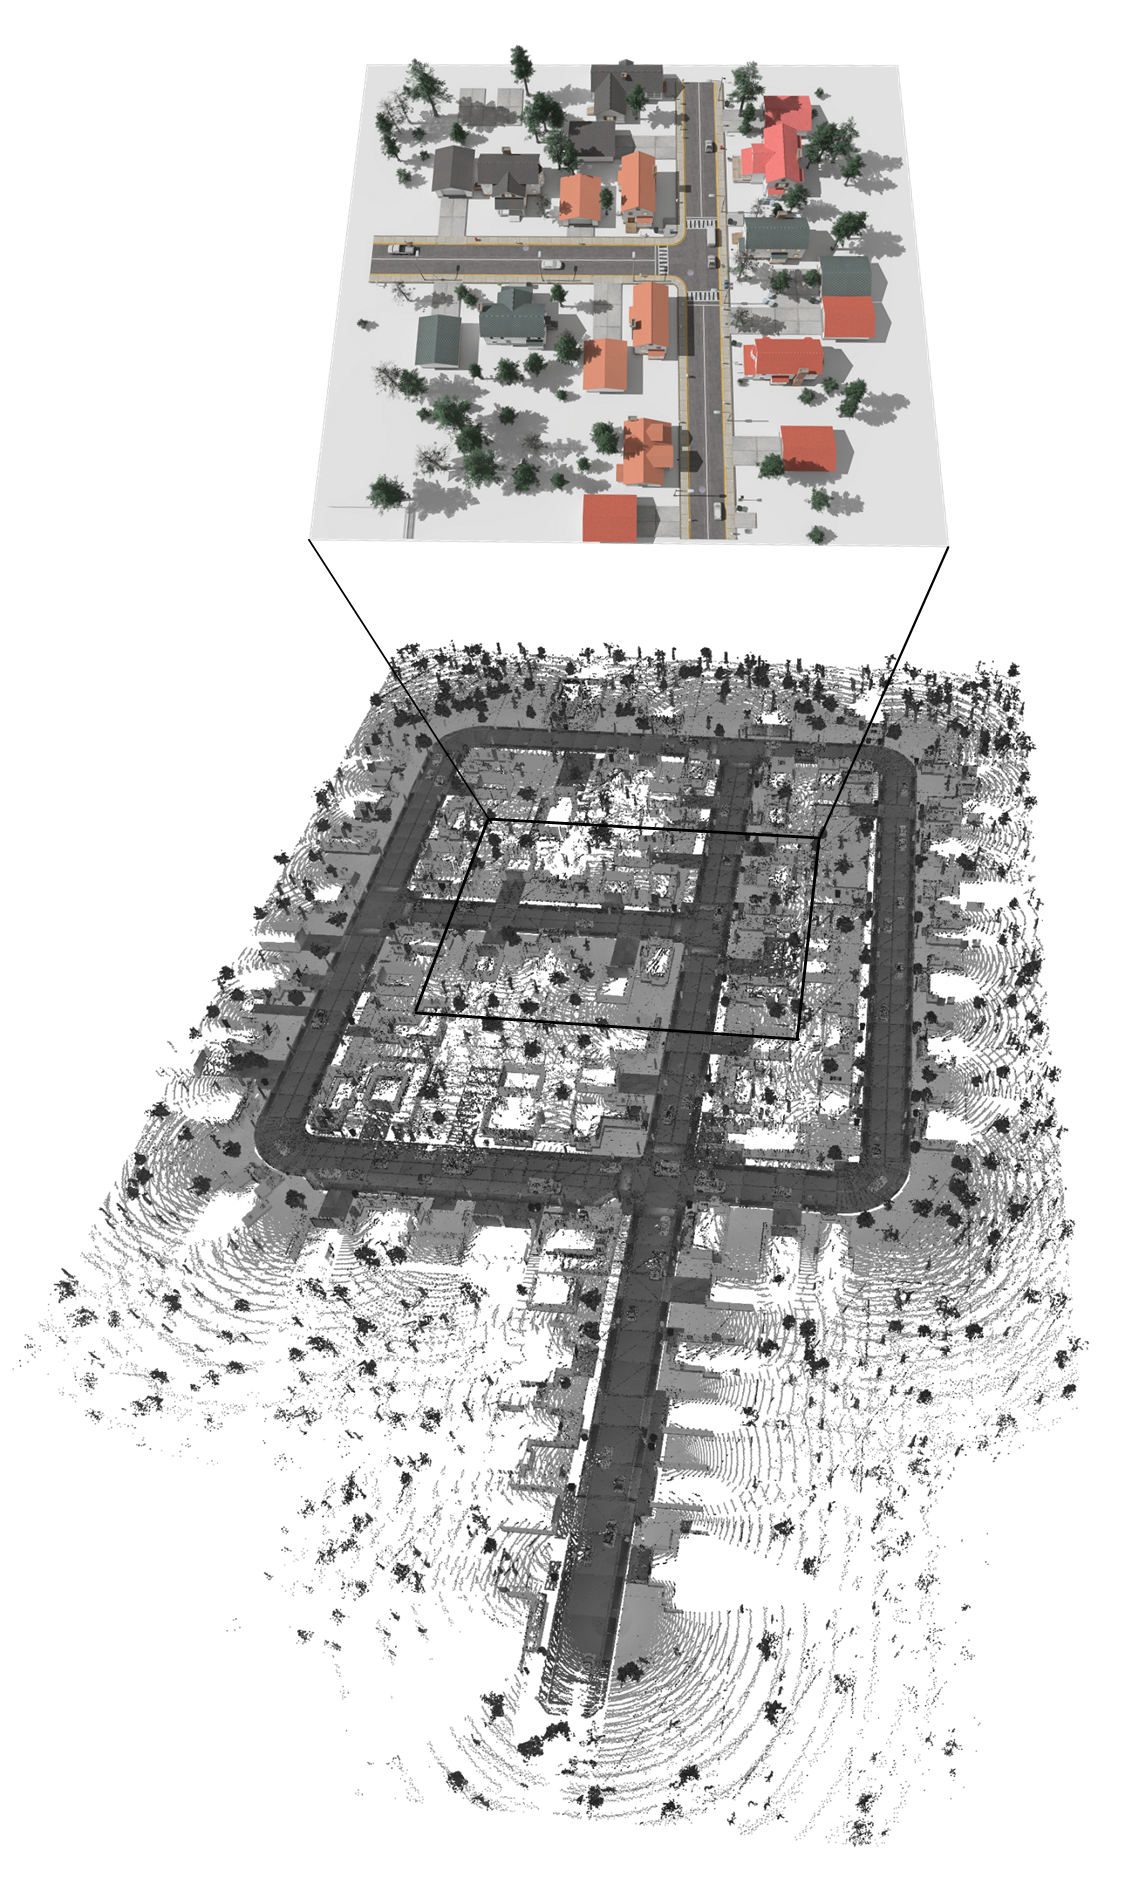
\includegraphics[width=\linewidth]{figs/lidar_intensity/material_database_intensity_results.png}
    \caption{\acrshort{lidar} intensity estimated over an urban scenario using the \acrshort{brdf}s collected with a goniphotometer.}
	\label{fig:lidar_material_database_intensity_result}
\end{marginfigure}
During the simulation, the data transferred to the \acrshort{gpu} was queried using $-\widehat{r_d}$, where $r_d$ is the ray direction. From here, the azimuth and elevation were calculated as shown in Equation \ref{eq:lidar_azimuth_elevation}. The reflectance was then accessed considering that data was stored in elevation-major order, with the indexing calculated as $m_{\textit{Id}} \cdot 360 \cdot 90 + \phi \cdot 90 + \theta$, with $m_{\textit{Id}}$ being the Id of the intersected material.
\begin{gather}
    \label{eq:lidar_azimuth_elevation}
    \begin{aligned}
        L &= -\widehat{r_d}\\
        \phi &= \lfloor{\abs{\arctan{\frac{L_y}{L_x}}} \cdot 180 \cdot \frac{1}{\pi} \rfloor}\\
        \theta &= \lfloor{\arccos{L_z} \cdot 180 \cdot \frac{1}{\pi} \rfloor}\\
    \end{aligned}
\end{gather}

Then, the obtained reflectance was integrated into the formulae of \acrshort{lidar}. The starting spectral signatures, depicted in Figure \ref{fig:brdf_merl_examples}, are weighted according to the dot product between the incident vector and the normal vector. An example of the intensity estimated during the scanning of an urban environment is illustrated in Figure \ref{fig:lidar_material_database_intensity_result}. 

\begin{figure}[hbt]
	\centering
	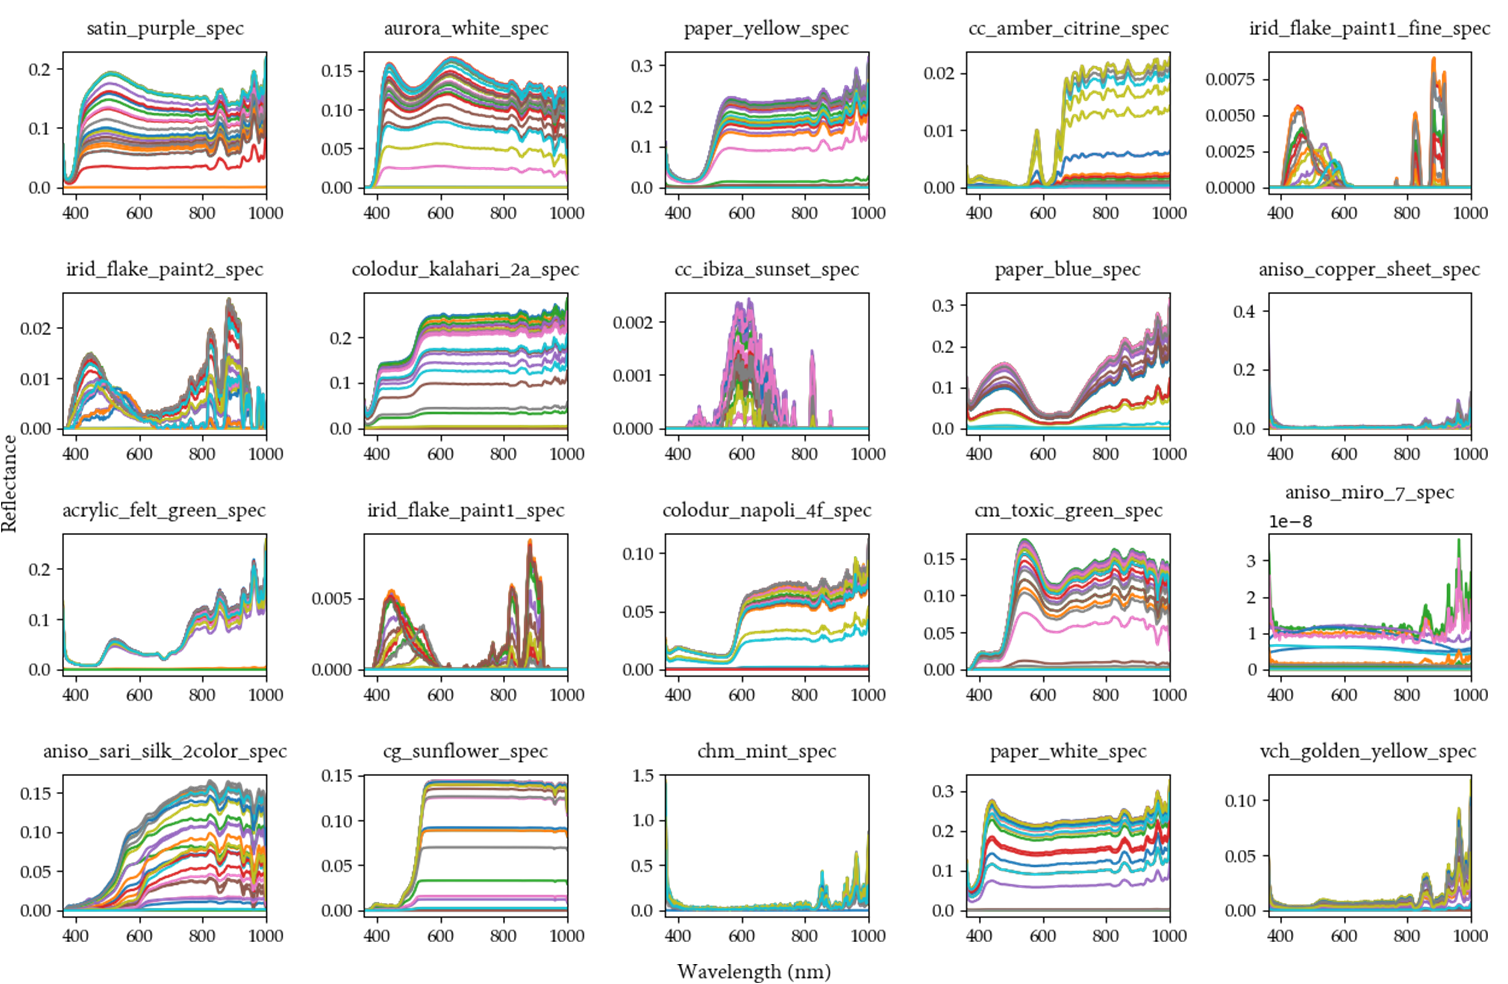
\includegraphics[width=.95\linewidth]{figs/lidar_intensity/brdf_database_examples.png}
	\caption{Signatures sampled from the material database published by Dupuy and Jakob \cite{dupuy_adaptive_2018}. Each cell represents a different material, and the depicted signatures are different samples for randomized input and output vectors. }
	\label{fig:brdf_merl_examples}
\end{figure}

\section{Results and discussion}

The proposed simulation was evaluated using the specifications of commercial \acrshort{lidar} sensors. Procedural scenes with a complexity ranging from 5M triangles to 11M were used as the input. The generated point clouds will be following analyzed to provide better insight into the estimation of intensity by changing the scene materials. During these experiments, the \acrshort{lidar} sensors were configured to return a single point per beam, whereas the rest of the properties were set according to the datasheets from Velodyne HDL-64E (\acrshort{tls}) and DJI Zenmuse L1 (\acrshort{als}) sensors. Still, the resolution and the vehicle speed were adjusted to have a considerable number of points. \acrshort{lidar}'s pulses were discretized using ten rays in every experiment.

\begin{figure}[ht]
	\centering
	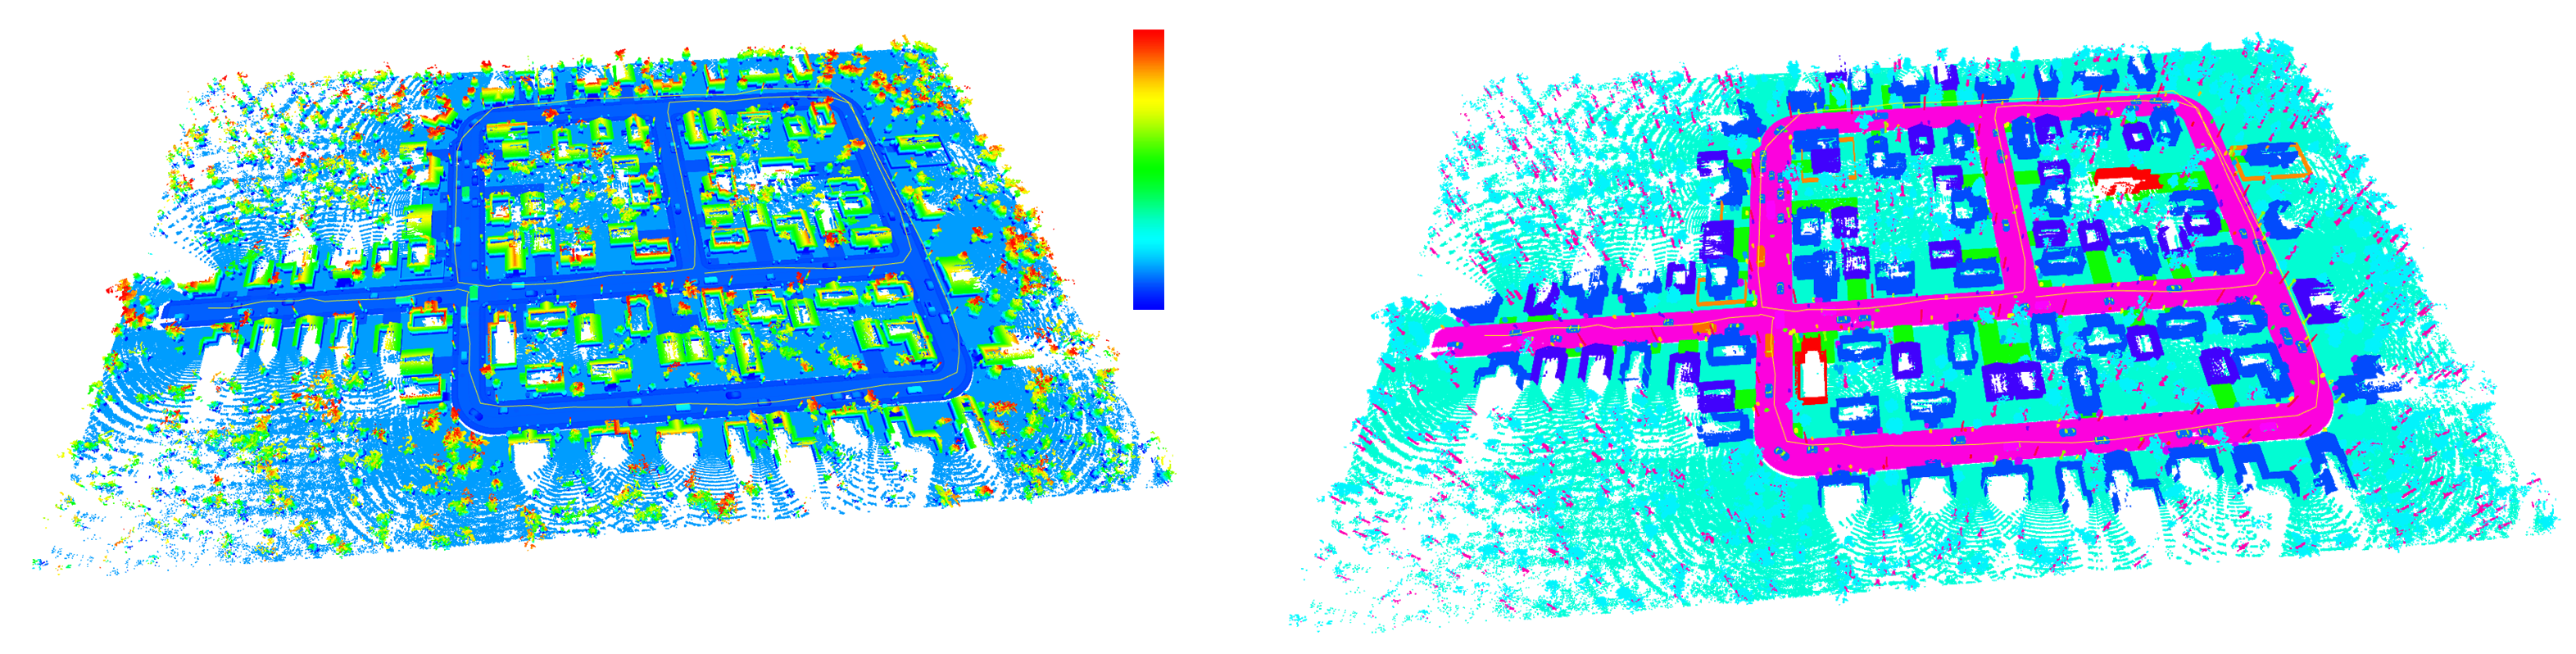
\includegraphics[width=\linewidth]{figs/lidar_intensity/experiment_scenarios.png}
	\caption{Point clouds obtained with a \acrshort{tls} simulation over an urban scenario. }
	\label{fig:lidar_intensity_experiment_scenario}
\end{figure}

\subsection{Analytical BRDFs}

The simulation of distinct surfaces is the main objective pursued by the proposed intensity estimation. Three different experiments were conducted to evaluate the outcome of analytical \acrshort{brdf}s. First, surfaces were modelled with the most appropriate material available in the database. According to this, the following materials and \acrshort{brdf}s were linked: \footnotesize\verb|Aluminium| $\gets$ \verb|Cook-Torrance|, \verb|Glass| $\gets$ \verb|Blinn-Phong|, \verb|Fabric| $\gets$ \verb|Minnaert|, \verb|Iron| $\gets$ \verb|Cook-Torrance|, \verb|Leaf| $\gets$ \verb|Oren-Nayar|, \verb|Plastic| $\gets$ \verb|Cook-Torrance|, \verb|Stone| $\gets$ \verb|Minnaert|, \verb|Wood| $\gets$ \verb|Ward Anisotropic|\normalsize. Then, every surface was modelled with the Lambertian \acrshort{brdf}. The returned intensity is depicted in Figure \ref{fig:database_intensity_lambertian_results}. Finally, the first setup was replicated for \acrshort{tls} and \acrshort{als} to illustrate the changes obtained using different scanning methods (see Figure \ref{fig:analytical_brdf_results}). The first two experiments were conducted over a procedural forestry environment, whereas the last one was performed over an urban scenario as the one shown in Figure \ref{fig:lidar_intensity_experiment_scenario}.

% The surfaces that were modelled with a dull-like appearance, e.g., leaf and fabric, returned lower intensity values. Furthermore, it is clear that is a strong correlation between the shape of the histograms and the type of scan. Airborne scans exhibit a Gaussian-like distribution as a consequence of covering a wider variety of surfaces, normal vectors and incidence angles. Note that the \acrshort{fov} in \acrshort{als} is also larger than in \acrshort{tls}, which is typically very narrow. As a consequence, terrestrial surveys have a lower variety of incidence angles that lead to a histogram with a completely different shape. The majority of values are gathered around zero rather than being uniformly distributed. However, changing the \acrshort{brdf}s to Lambertian contributed to obtaining more uniform intensity distributions. The surfaces that were initially modelled with Minnaert \acrshort{brdf} increased significantly the returned intensity after this change, and the contrary occurred for \acrshort{brdf}s that returned higher intensity at first. 

Surfaces with a dull appearance, such as leaves and fabric, returned lower intensity values compared to other surfaces. Additionally, a strong correlation was found between the shape of the intensity histograms and the type of scan. Airborne scans exhibit a Gaussian-like distribution due to the wider variety of surfaces, normal vectors, and incidence angles covered. It is worth noting that the \acrshort{fov} in \acrshort{als} is typically larger than in \acrshort{tls}, which contributes to a greater variety of incidence angles and therefore achieves a histogram with a different shape. In contrast, terrestrial surveys have a narrower \acrshort{fov} and a lower variety of incidence angles, leading to a histogram with most values gathered around zero instead of being uniformly distributed.

It was also observed that changing the \acrshort{brdf}s to Lambertian resulted in more uniform intensity distributions. Specifically, surfaces that were initially modelled with Minnaert \acrshort{brdf} showed a significant increase in returned intensity after this change, while the opposite occurred for \acrshort{brdf}s that initially returned higher intensity values.

\begin{figure*}[ht]
	\centering
	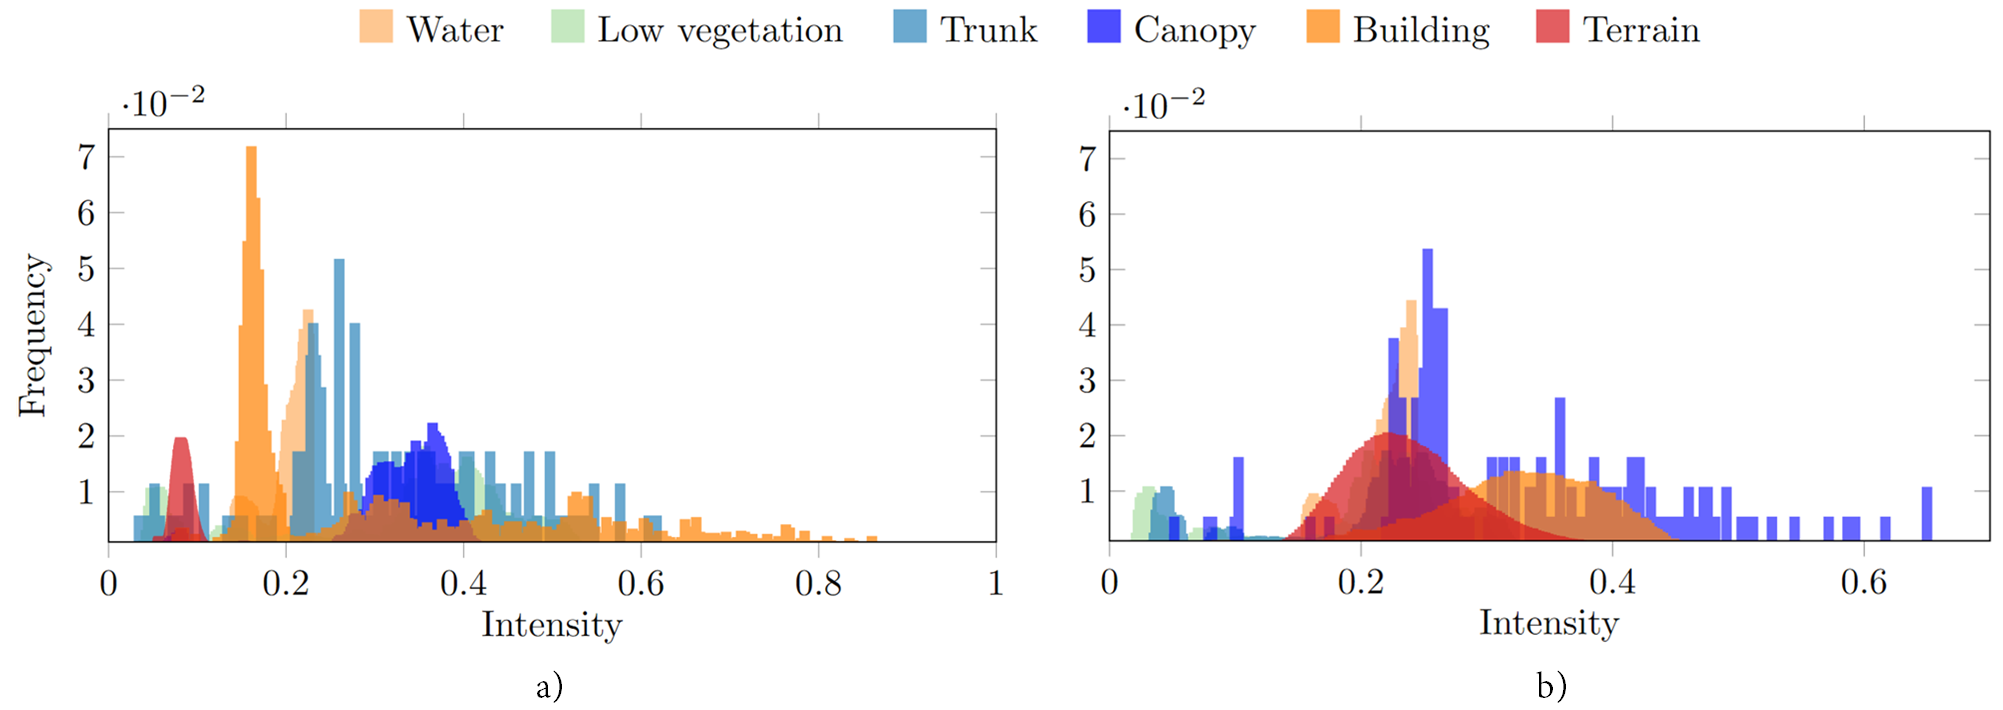
\includegraphics[width=\linewidth]{figs/lidar_intensity/analytical_intensity_lambertian.png}
	\caption{Comparison of the intensity estimated in the aerial scanning of a procedural forestry environment. a) Objects were modelled with a \acrshort{brdf} similar to the expected appearance, whereas b) uses a Lambertian \acrshort{brdf} for every surface.  }
	\label{fig:database_intensity_lambertian_results}
\end{figure*}

\begin{figure*}[ht]
	\centering
	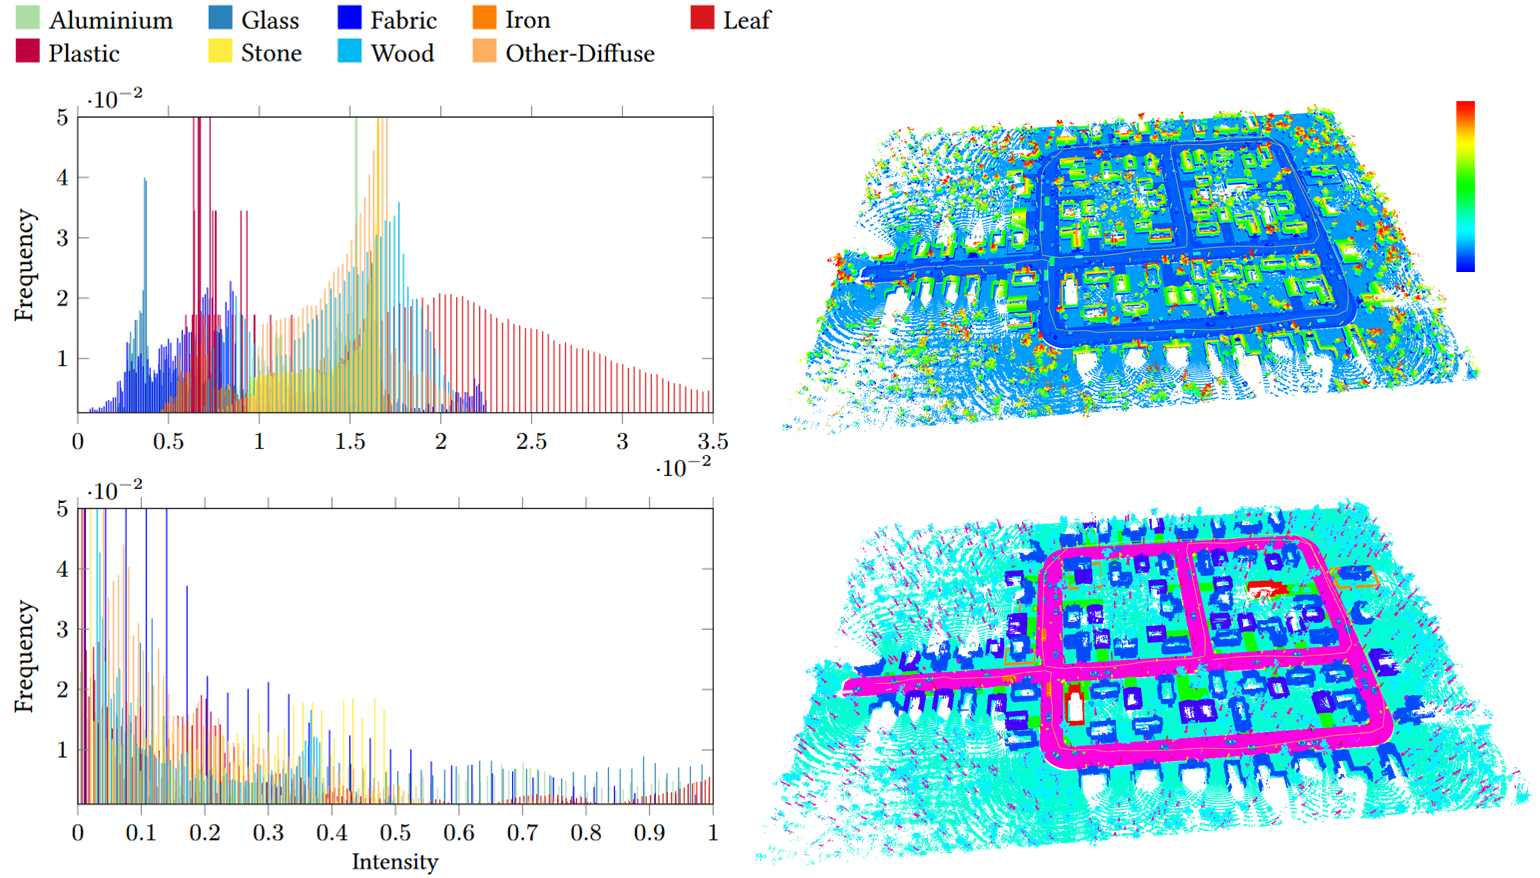
\includegraphics[width=\linewidth]{figs/lidar_intensity/analytical_brdf_intensity_chart.png}
	\caption{Comparison of intensity estimated from a) airborne and b) terrestrial scans. }
	\label{fig:analytical_brdf_results}
\end{figure*}

% Regarding .  distribution of intensity over $[0, 1]$ varies depending both on the surface \acrshort{brdf} and the normal vector. Hence, histograms from aerial surveys show a Gaussian form, since a wider variety of normal vectors are sampled. On the other hand, terrestrial results are more unbalanced as a result of a narrow field of view. Using only Lambertian surfaces, the intensity values are more uniformly distributed, although histograms vary as a consequence of distance and observed normals. However, similarly to Figure \ref{fig:analytical_brdf_results}, materials following diffuse \acrshort{brdf}s, e.g. Minnaert, present a brighter signature when represented as Lambertian.

\subsection{BRDF database}

Using this approach, the experiments were conducted by changing 1) the sensor wavelength from 903 \si{\nano\meter} to 532 \si{\nano\meter}, thus expecting a lower intensity in the latter configuration, and 2) the surface materials. First, all the surfaces were modelled with \acrshort{brdf}s similar to the expected appearance, ranging from acrylic to metallic and anisotropic profiles, and then, all of them were modelled the \acrshort{brdf} extracted from a maple leaf, which offers a similar outcome to the Lambertian \acrshort{brdf}. The outcome of the three conducted experiments is illustrated in Figure \ref{fig:database_intensity_results}. 

\begin{figure*}[ht]
	\centering
	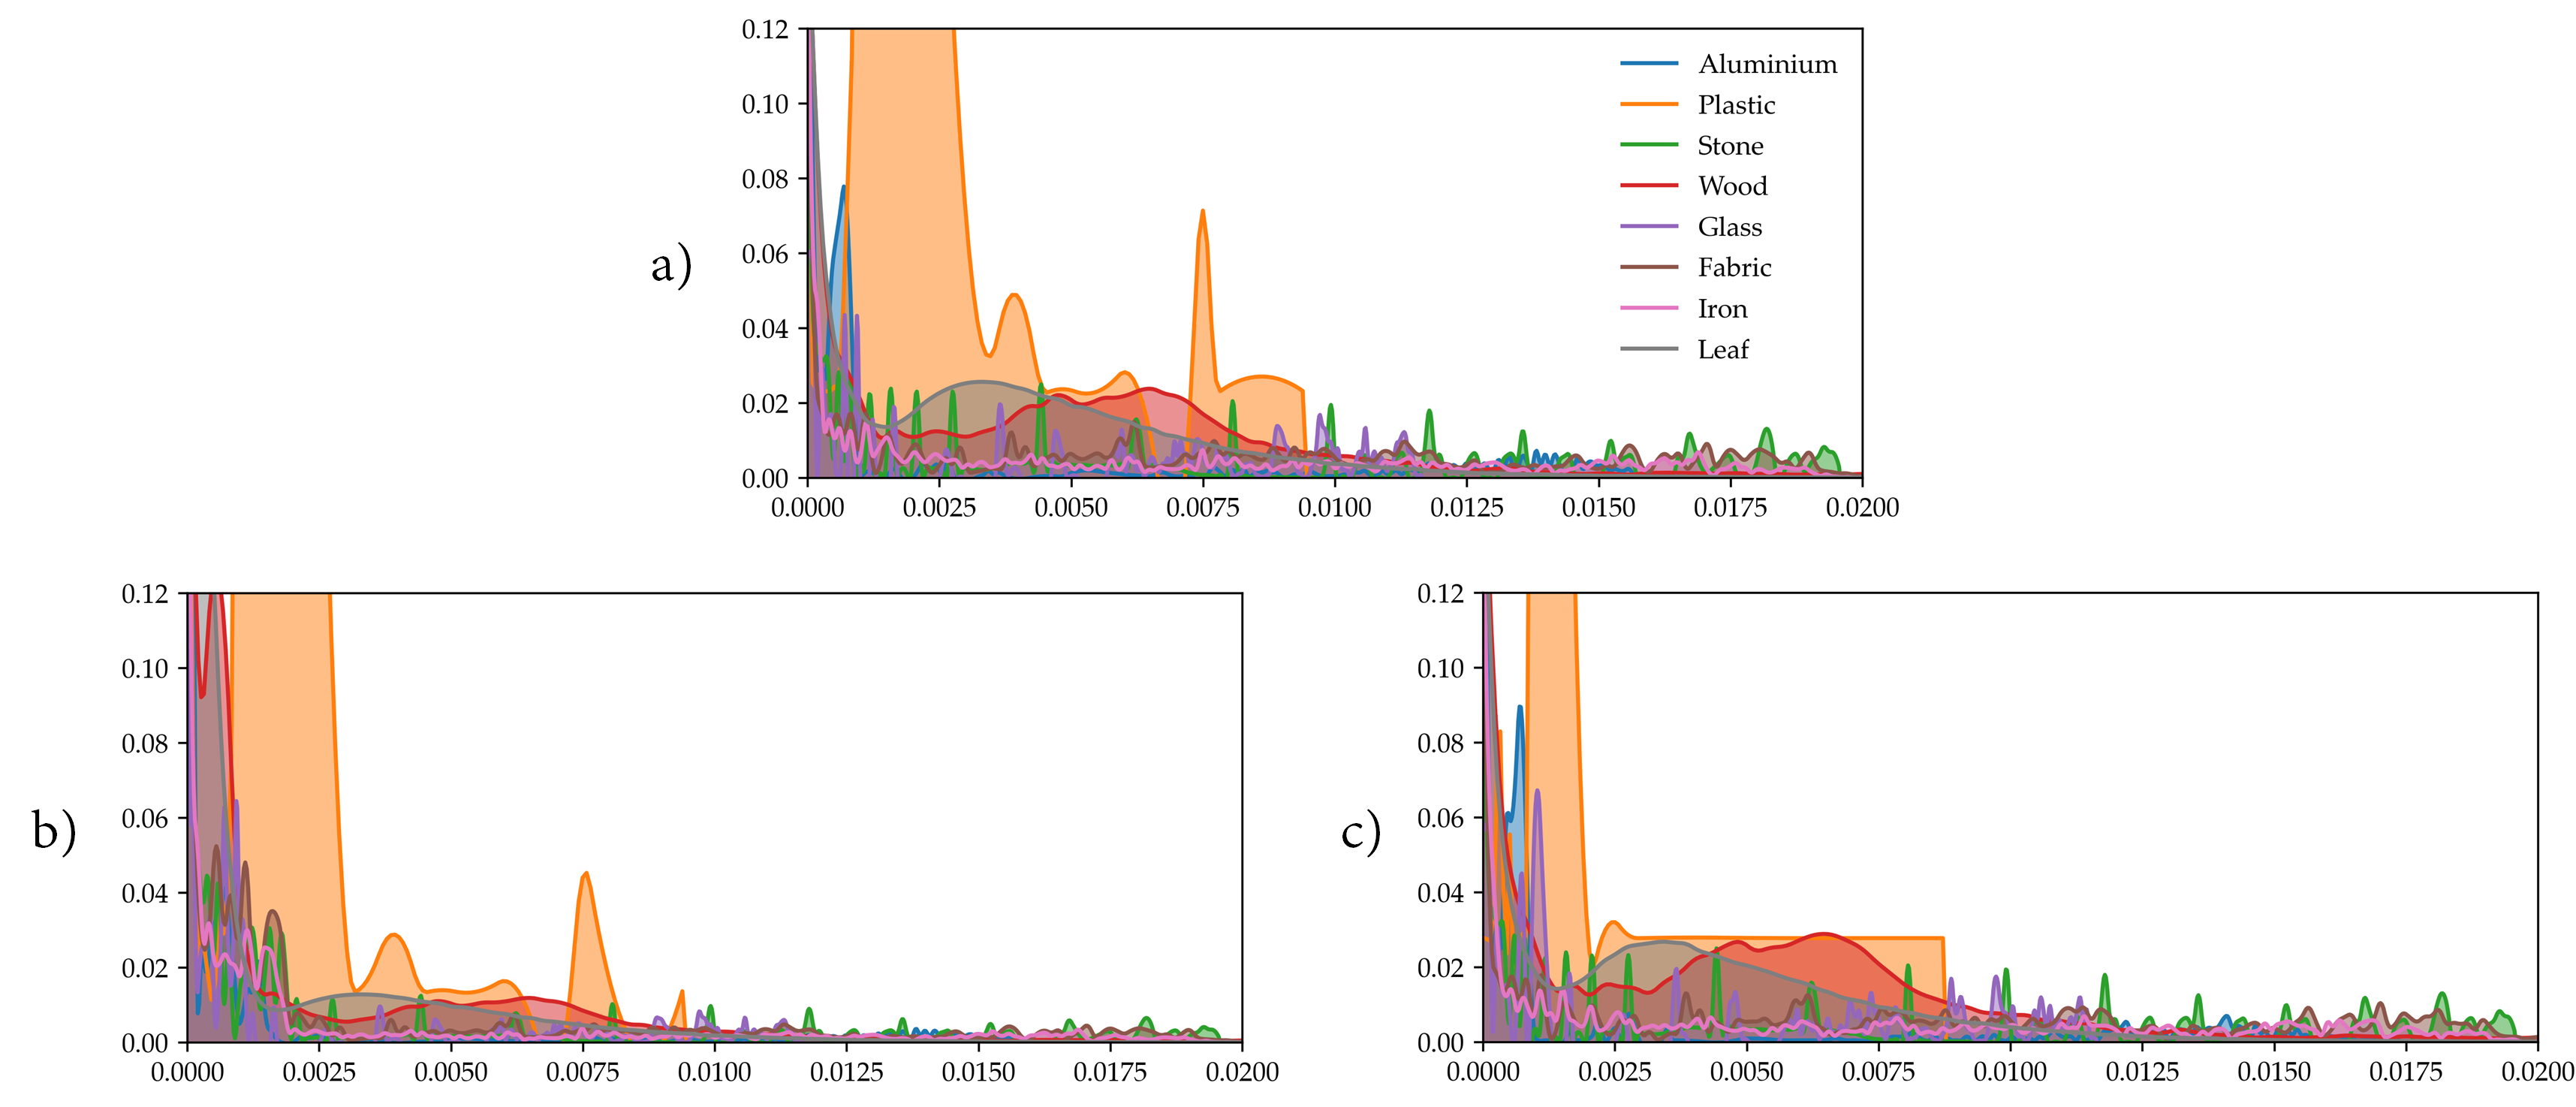
\includegraphics[width=\linewidth]{figs/lidar_intensity/database_intensity_chart.png}
	\caption{a) intensity from the simulation of an HDL-64E \acrshort{lidar} operating at 903 \si{\nano\meter} over surfaces with realistic materials, b) idem but working at 532 \si{\nano\meter} and c) the first experiment replicated with Lambertian surfaces. }
	\label{fig:database_intensity_results}
\end{figure*}

The intensity histograms of our \acrshort{tls} scans are strongly influenced by both the wavelength of the \acrshort{lidar} and the materials present in the scene. Because our scans were conducted with a narrow \acrshort{fov}, most of the returned intensity values are close to zero, since the incident vector and the majority of surfaces have different orientations. This is in contrast to scans performed from a terrestrial vehicle, which reach a large number of surfaces oriented such that $\hat{n} = -\hat{r_d}$ (where $n$ is the surface normal and $r_d$ is the ray direction). However, the long-range capabilities of our \acrshort{lidar} allow us to detect very distant surfaces with normal vectors that differ significantly from $r_d$, which in turn diminishes the returned intensity. Interestingly, we found that changing the \acrshort{lidar} wavelength from 532 \si{\nano\meter} to 903 \si{\nano\meter} increased the returned intensity. This result was expected by observing Figure \ref{fig:brdf_merl_examples} since the majority of materials have signatures that grow as the wavelength increases. Furthermore, using a single \acrshort{brdf} intended to emulate a Lambertian response led to overall brighter intensity values. However, it is important to note that this configuration does not necessarily imply upscaling of intensity values. Instead, this approach offers a mid-range intensity that is lower than the signature of some materials but brighter than materials with a dull appearance.

\section{Conclusions and future work}

Two different methodologies were evaluated for estimating the \acrshort{lidar} intensity during scans solved in the \acrshort{gpu}. The first one uses traditional shading methods, where \acrshort{brdf}s were expressed using formulae intended to emulate the appearance of any material. However, only six analytical \acrshort{brdf}s were implemented, thereby evidencing that it is not possible to cover every material found in nature. Additionally, not all of these \acrshort{brdf}s are physically based, and selecting one over another can be challenging. For instance, there are several \acrshort{brdf}s that emulate anisotropic materials. Another approach is to obtain \acrshort{brdf}s by sampling real-world materials using a gonio-photometer \cite{dupuy_adaptive_2018}. This method is based on the sampling of published \acrshort{brdf} databases which provide more reliable signatures and extend the spectra from \acrshort{rgb} to a wider wavelength range. Also, using collected \acrshort{brdf}s eliminates parameters used to estimate the reflectance from scratch (e.g., specular colour). Therefore, this approach was proven to be much more convenient, whereas the obtained results did not show any notable changes compared to the first approach. Indeed, the conducted \acrshort{tls} scans had a very similar intensity distribution.

% Following the work of the previous chapter, the simulated point clouds, together with the estimated density, ought to be evaluated in \acrshort{dl} to either prove their degree of applicability or adjust the process whether it is required. Also, including the intensity in other kinds of sensors, such as full-waveform \acrshort{lidar} \cite{tachella_real-time_2019}, would be of great interest.

Building on the previous chapter's work, it is essential to evaluate the simulated point clouds, along with the estimated density, using \acrshort{dl}. This evaluation will help determine the degree of applicability of the simulated data and enable any necessary adjustments to the process. Additionally, integrating intensity data to other kinds of sensors, such as full-waveform \acrshort{lidar} \cite{tachella_real-time_2019}, would be highly beneficial to expand the scope of this research.